\section{Manipulation 1 "Mesurer la vitesse de propagation du son dans des
barreaux solides par méthode de résonance en mode continu."}
\subsection{\large Approches / Méthodes}
\subsubsection{\large Rappels Théoriques}

\paragraph{Introduction}
De manière générale, une onde se propage dans toutes les directions
qui lui sont offertes à partir de sa source. Si nous prenons l'exemple
d'une personne qui parle, cela représente une onde progressive à trois 
dimensions. Si on imagine une fine feuille de métal, que l'on vient
frapper avec un marteau, les ondes générées au point d'impact vont 
se propager que dans le plan, on aura une onde progressive à deux 
dimensions. \\
Dans ce rapport, nous allons nous limiter à la propagation 
unidimensionnelle.
Illustrons ceci avec l'exemple d'une corde tendue, le long de 
laquelle une onde se propage (voir Figure 1). Cette onde n'a qu'une 
direction qui lui est offerte. Nous allons nous restreindre à une onde 
dite progressive, la perturbation ne se déforme pas lors de 
sa propagation.~\cite{propagation-onde}
%Cette onde est dépendante d'une variable de position et d'une variable 
%de temps.~\cite{revisions-bac-unidimensionnel} \\
La direction de propagation de la perturbation se trouve dans la direction
de l'axe des abscisses, nommée $"x"$, selon la Figure 1.
Une onde 1D se propageant s’écrit comme une fonction dépendante 
de la position x et du temps t : $y(x, t)$, ces deux variables donnent le 
profile de l'onde.
Une onde ne se propage pas instantanément, elle a une vitesse également appelée célérité
finie et il faut donc un certain temps pour qu’une perturbation atteigne
un point donné de l’espace.
La forme de la perturbation initiale, cette fonction se retrouve identique
à elle-même, mais décalée dans l’espace à un instant t > 0. 
La question est de combien est-elle décalée ? L’onde se propageant à la célérité $c$, 
après un temps $t$ on retrouve la perturbation translatée 
d’une distance $ct$.~\cite{propagation-onde}
%la fonction est décrite selon 
%deux variables qui donnent le profile de l'onde, en fonction de la 
%position et du temps, soit $y(x ; t)$. 
C'est donc sur un modèle similaire 
que nous allons effectuer nos mesures.

%\begin{figure}[h]
%    \centering
%    \adjustbox{max width=\textwidth}{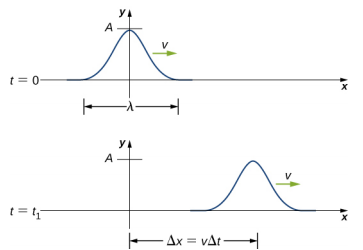
\includegraphics{onde.png}}
%    \caption{Onde progressive à une dimension.~\cite{image-onde-progressive}}
%\end{figure}

\begin{figure}[h]
    \centering
    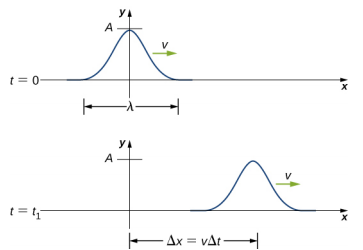
\includegraphics[width=10cm]{onde.png}
    \caption{Onde progressive à une dimension.~\cite{image-onde-progressive}}
\end{figure}

\newpage

La célérité est indépendante de l'intensité 
de l'onde. On note toutefois des exceptions lorsque la perturbation 
du milieu est violente, où les variations sont de l'ordre de la densité 
moyenne du milieu.~\cite{pastur-onde}\\

Autrement dit, la célérité d’une onde ne dépend pas de son amplitude 
tant qu’elle reste "raisonnable".
%tant qu'elle ne change pas les caractéristiques du milieu 
%de propagation.
Dans ce cas la célérité 
est une caractéristique du milieu qui est dite linéaire.
On considérera des milieux dans lesquels la célérité d’une onde 
est indépendante de la forme de celle–ci, on dit que le milieu est
non–dispersif.\\
La célérité d’une onde dépend de la nature de celle–ci, 
dans un même milieu une onde longitudinale ou transversale n’a pas même
célérité. \\
%\footnote{LUC PASTUR. 
%\textit{Ondes et Accoustiques dans les FLuides --- Université Paris-Saclay}. 
%[en ligne]. 2017. [consulté le 17.10.2023]. Disponible sur : 
%\href{https://perso.limsi.fr/pastur/meca/M1MFL_oaf.pdf}
%{perso.limsi.fr}}\\
Dans le cas de l’acoustique, c’est une onde de pression qui se propage 
(une succession de surpression et de dépression) mais elle est également 
associée à une vitesse locale des particules composant le milieu de 
propagation.

La célérité de l'onde reste constante, tant que les caractéristiques 
du milieu de propagation ne changent pas ni en fonction du temps, 
ni en fonction de la position. 

La vitesse ne dépend que des caractéristiques du milieu.
Cette vitesse est proportionnelle entre la distance et le temps.

La célérité est homogène à une vitesse, mais on réservera le mot vitesse 
à un déplacement de matière et célérité à la vitesse de propagation 
d’une onde. \\
D’après nos hypothèses, la célérité d’une onde est donc uniquement 
dépendant des caractéristiques, du milieu de propagation et éventuellement 
de la nature de l’onde.

Dans le cas d’une onde qui se propage, la perturbation du milieu dépend 
de la position et du temps.\\

Nous allons également utiliser le phénomène de résonance d'un matériau 
lors de cette expérience. Ce qui nous permettra d'avoir sur une prise de 
mesure continue, une amplitude maximale et stable dans le temps.

%Une onde 1D se propageant s’écrit comme une fonction dépendante 
%de la position x et du temps t : s(x, t).
%Une onde ne se propage pas instantanément, elle a une célérité 
%finie et il faut donc un certain temps pour qu’une perturbation atteigne
%un point donné de l’espace.
%La forme de la perturbation initiale, cette fonction se retrouve identique
%à elle même mais décalée dans l’espace à un instant t > 0. La question est, 
%de combien est–elle décalée ? L’onde se propageant à la célérité c, 
%après un temps t on retrouve la perturbation translatée d’une distance $ct$.~\cite{propagation-onde}

\newpage

\paragraph{Equations physiques}
\begin{align}
    \intertext{La célérité d'une onde progressive s'écrit :}
    c &= \frac{dx}{dt} = \frac{x_2 - x_1}{t_2 - t_1}\\
    \intertext{L'expression mathématique d'une onde progressive 1D 
    se propageant le long de l'axe $Ox$ dans le sens des $x$ croissant et 
    à la célérité $c$ peut s'écrire :}
    s(x, t) &= f(x - ct) \notag \\
    &= f\left(x - \frac{x}{c}\right)
    \intertext{L'expression mathématique d'une onde progressive 1D 
    se propageant le long de l'axe $Ox$ dans le sens des $x$ décroissant et 
    à la célérité $c$ peut s'écrire :}
    s(x, t) &= f(x + ct) \notag \\
    &= f\left(x + \frac{x}{c}\right)
    \intertext{Onde plane progressive harmonique: L'expression mathématique 
    d'une onde progressive 1D se propageant le long de l'axe $Ox$ dans le 
    sens des $x$ croissant et à la célérité $c$ peut s'écrire :}
    s(x, t) &= f(x - ct) \notag \\
    &= A\cos(\omega(t-\frac{x}{c}) + \phi) \notag \\
    &= A\cos(\omega t - kx + \phi)
    \shortintertext{ $A$ Amplitude maximale de l'onde}
    \shortintertext{ $\phi$ Le déphasage de l'onde}
    \shortintertext{La pulsation temporelle nommée $\omega$: }
    \omega &= 2\pi f = \frac{2\pi}{T}
    \shortintertext{ $f$ la fréquence de l'onde}
    \shortintertext{ $T$ la période de l'onde}
    \shortintertext{La pulsation spatiale ou nombre d'onde nommée $k$: }
    k &= \frac{\omega}{c} = \frac{2\pi f}{c} = \frac{2\pi}{\lambda}
    \shortintertext{ $\lambda$ la longueur d'onde de l'onde} \notag
\end{align}
\newpage
\begin{align}
    \shortintertext{ Evolution temporelle d'un point donné du milieu:}
    \shortintertext{La période:}
    T &= \frac{\lambda}{c}
    \shortintertext{La fréquence:}
    f &= \frac{1}{T}
    \shortintertext{La pulsation:}
    \omega &= 2\pi f
    \intertext{ Evolution spatiale du milieu à un instant donné:}
    \shortintertext{La période:}
    \lambda &= cT
    \shortintertext{La fréquence:}
    \kappa &= \frac{1}{\lambda}
    \shortintertext{La pulsation:}
    k &= 2\pi\kappa
\end{align}

\begin{figure}[h]
    \centering
    \begin{minipage}{0.45\textwidth}
        \centering
        \adjustbox{max width=\linewidth}{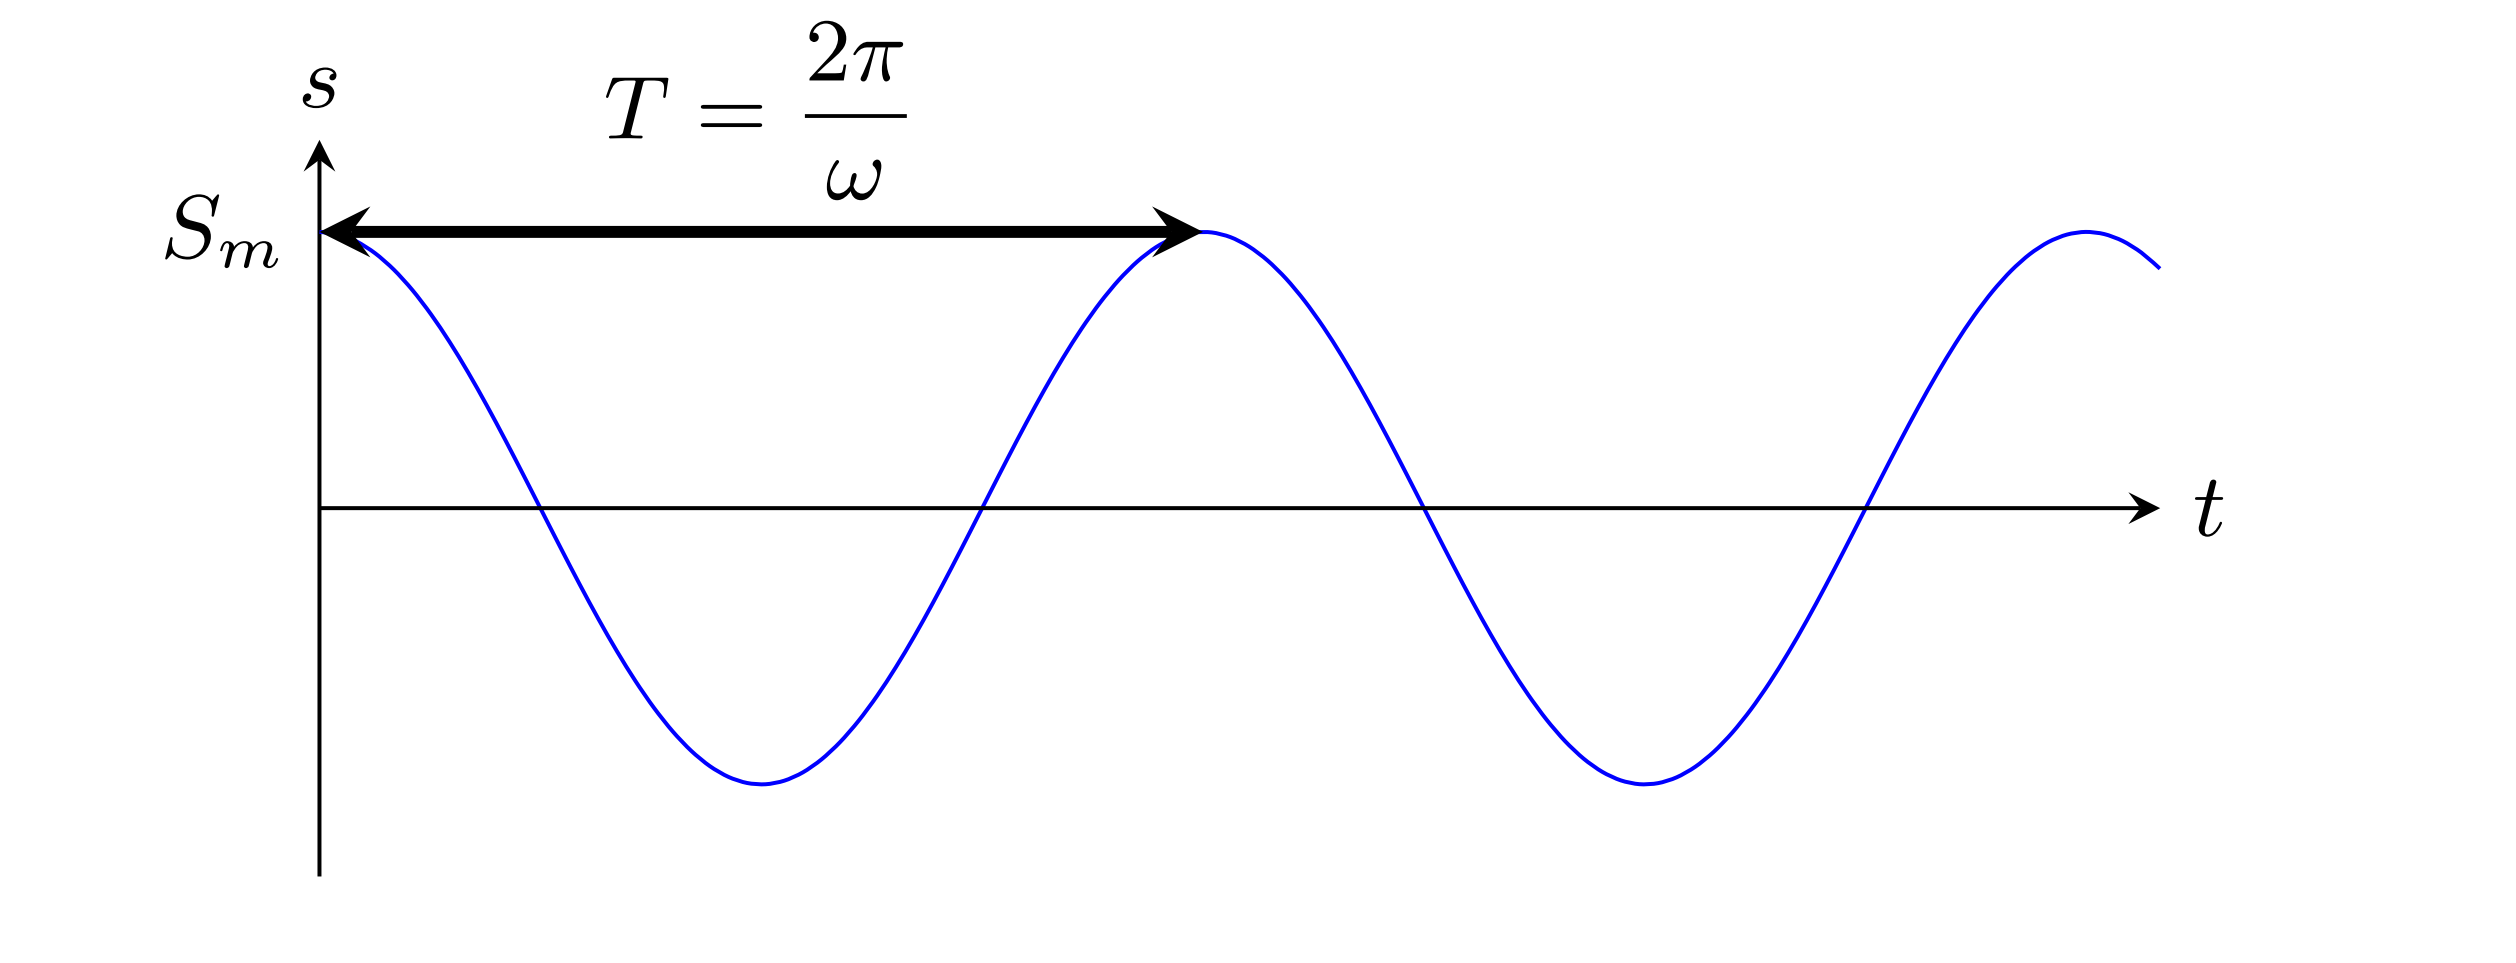
\includegraphics{evolution_temporelle.png}}
        \caption{Evolution temporelle d'un point donné du milieu.~\cite{propagation-onde}}
    \end{minipage}
    \hfill
    \begin{minipage}{0.45\textwidth}
        \centering
        \adjustbox{max width=\linewidth}{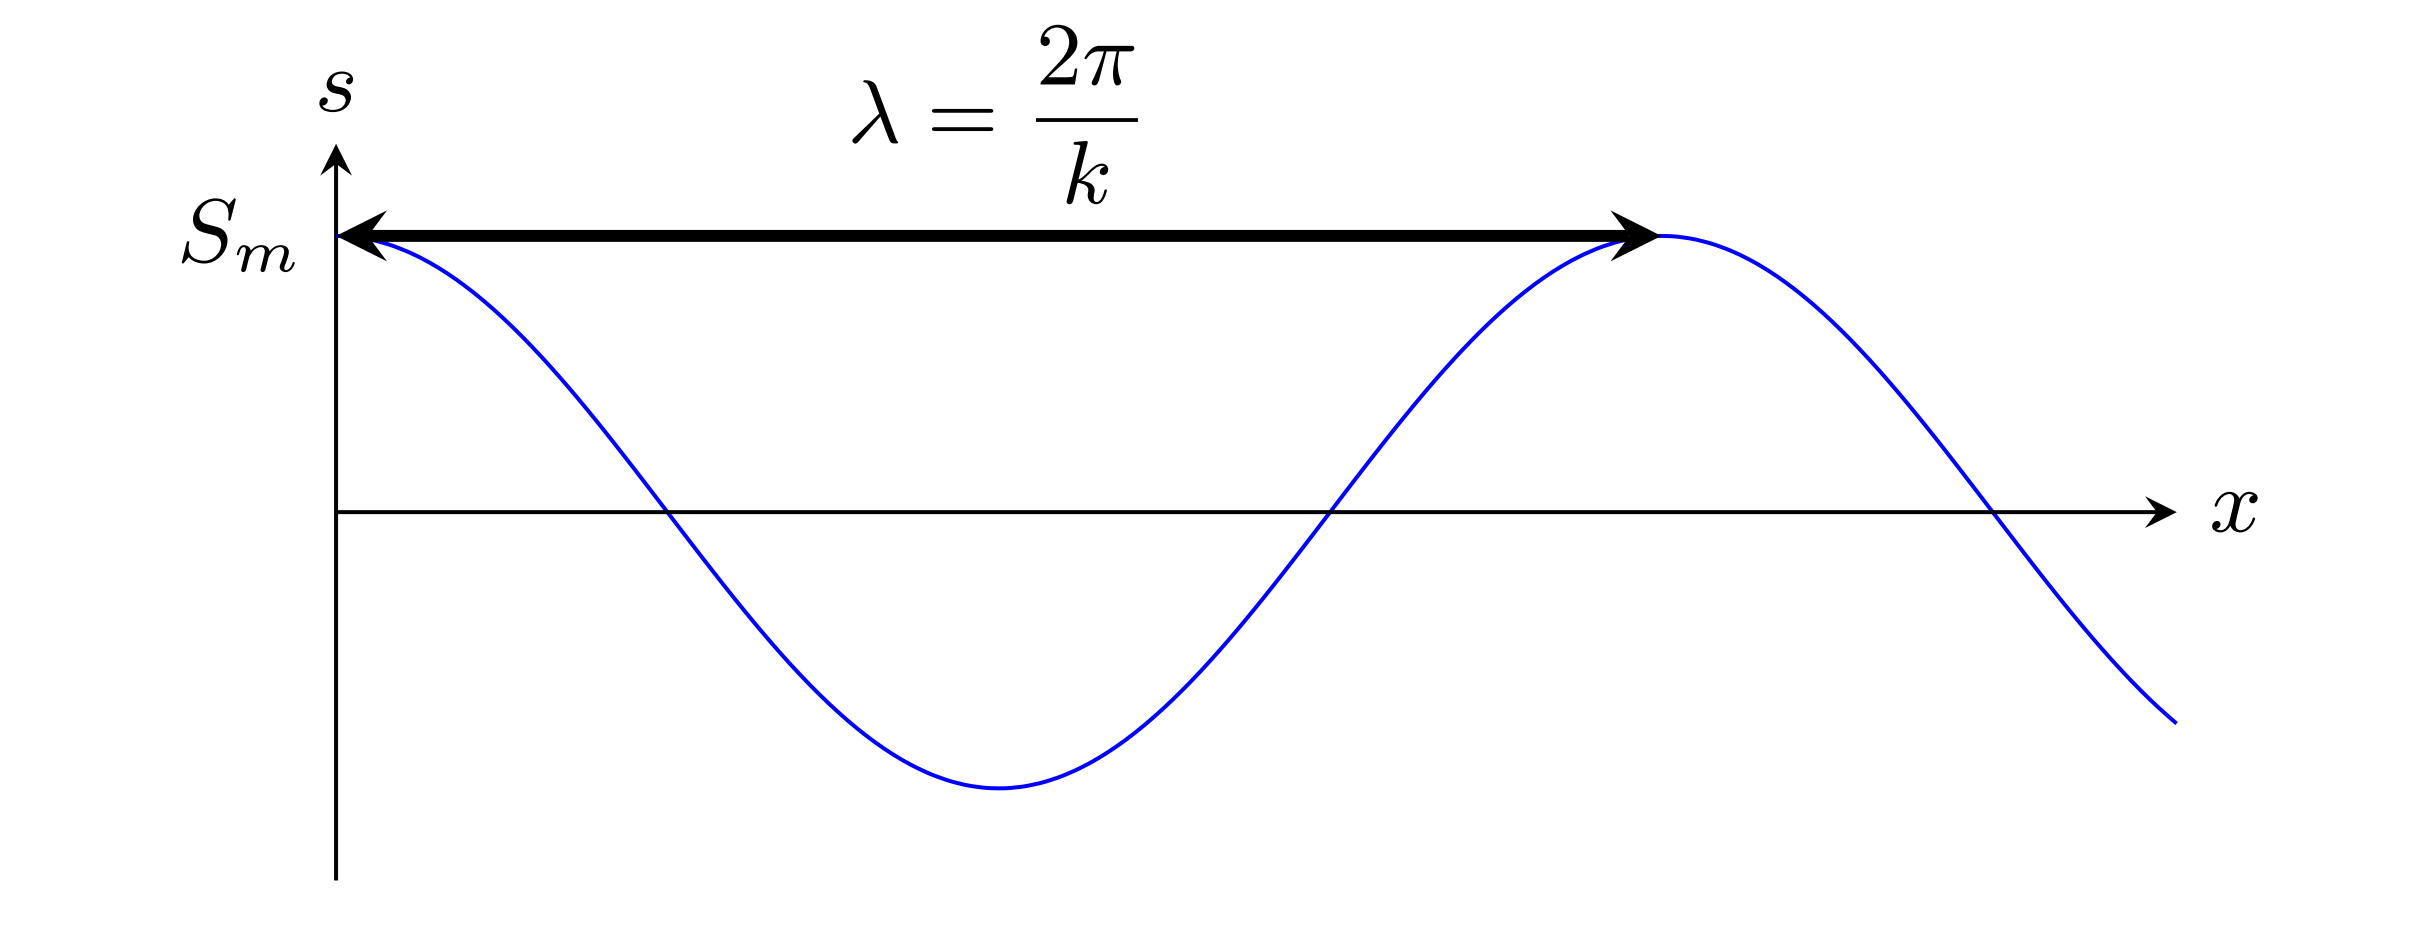
\includegraphics{evolution_spatiale.png}}
        \caption{Evolution spatiale du milieu à un instant donné.~\cite{propagation-onde}}
    \end{minipage}
\end{figure}

Nous allons donc pouvoir déterminer la célérité 
en passant également par l'onde plane progressive harmonique en tournant 
notre équation de la manière suivante :
\begin{align}
    \shortintertext{La célérité d'une onde s'écrit:}
    c &= \lambda f
    %\shortintertext{ La célérité d'une onde peut aussi s'exprimer de la 
    %manière suivante (ceci va nous permettre de trouver notre fréquence 
    %de résonance de notre matériau)}
    %c  &= \sqrt{\frac{E}{\rho}}
    %\shortintertext{ $ \rho$ la masse volumique $[\frac{kg}{m^3}]$}
    %\shortintertext{ $ E$ le module de Young du solide $[Pa]$} \notag
    %\shortintertext{ En prenant l'équation (1) et (8) nous pouvons déterminer la fréquence:}
    %c &= \frac{2d}{T} \Leftrightarrow T = \frac{2d}{c} \Leftrightarrow f = \frac{c}{2d}
    %\shortintertext{ $d$ est la longeur de l'échantillon $[m]$}\notag
\end{align}

\newpage

\begin{align}
    \shortintertext{ La célérité d'une onde peut aussi s'exprimer de la 
    manière suivante (ceci va nous permettre de trouver notre fréquence 
    de résonance de notre matériau):}
    c  &= \sqrt{\frac{E}{\rho}}
    \shortintertext{ $ \rho$ la masse volumique $[\frac{kg}{m^3}]$}
    \shortintertext{ $ E$ le module de Young du solide $[GPa]$} \notag
    \shortintertext{ En prenant l'équation (1) et (8) nous pouvons déterminer la fréquence:}
    c &= \frac{dx}{dt} \Leftrightarrow c = \frac{2d}{T} \Leftrightarrow T = \frac{2d}{c} \Leftrightarrow f = \frac{c}{2d} \Leftrightarrow f = \frac{\sqrt{\frac{E}{\rho}}}{2d}\\ \notag
    \shortintertext{ $d$ est la longeur de l'échantillon $[m]$}\notag
    \shortintertext{ Nous anticipons selon notre montage (voir Figure 4)
    qu'une période est mesuré par le microphone tous les $dx = 2d$}\notag
\end{align}

%\paragraph{Liste des paramètres}
\paragraph{Calculs d'incertitudes}
La propagation d'incertitude basée sur le cours IPH est calculé de la manière 
suivante :~\cite{gravier-laurent}\\[2ex]
Relation :
\begin{align}
    g &= f(a) \\
    \Delta g &= |\frac{\partial f}{\partial a}|\Delta a + |\frac{\partial f}{\partial b}|\Delta b + |\frac{\partial f}{\partial c}|\Delta c + \ldots
\end{align}
L'incertitude $\Delta g$ est arrondi à 1 chiffre significatif selon le cours 
IPH.\\[2ex]
a, b, c sont les grandeurs physiques mesurées de manière directe. \\[2ex]
$\Delta a, \Delta b, \Delta c$ sont les incertitudes absolues des grandeurs 
a,b,c.\\[2ex]
$|\frac{\partial f}{\partial a}|;|\frac{\partial f}{\partial b}|;|\frac{\partial f}{\partial c}|$
sont les dérivées partielles de B par rapport à a, b, c.\\
\begin{align}
    \shortintertext{ Dans notre cas, la première méthode de mesure 
    nous donne une incertitude:}\notag\\
    \Delta c &= c \left( \frac{\Delta x}{x} + \frac{\Delta t}{t} \right) \\[2ex]
    \shortintertext{ $\Delta x$ $\pm$ 2 mm (valeur à ajuster)}
    \shortintertext{ $\Delta t$ $\pm$ 500 ms (valeur à ajuster)}\notag \\
    \shortintertext{ La deuxième méthode de mesure nous donne 
    une incertitude:}\notag  \\
    \Delta c &= c \left( \frac{\Delta \lambda}{\lambda} + \frac{\Delta f}{f} \right) \\[2ex] \notag 
    \shortintertext{ $\Delta \lambda$ $\pm$ 1 mm (valeur à ajuster)}
    \shortintertext{ $\Delta f$ $\pm$ 5 Hz (valeur à ajuster)} \notag
    \shortintertext{ L'équation (14) nous donne une incertitude:}
    \Delta c &= \frac{c}{2} \left( \frac{\Delta E}{E} + \frac{\Delta \rho}{\rho} \right)
    \shortintertext{ $\Delta E$ $\pm$ 10 $GPa$ (valeur à ajuster, sera prise d'internet)}
    \shortintertext{ $\Delta \rho$ $\pm$ 2 $\frac{kg}{m^3}$ (valeur à ajuster, sera prise d'internet)} \notag
    \shortintertext{ L'équation (15) nous donne une incertitude:}
    \Delta f &= f \left( \frac{\Delta c}{c} + \frac{\Delta d}{d} \right) \\[2ex]
    \shortintertext{ $\Delta c$ $\pm$ 2 $\frac{m}{s^2}$ (valeur à ajuster)}
    \shortintertext{ $\Delta d$ $\pm$ 1 mm (valeur à ajuster)}\notag \\
\end{align}

\newpage

\subsubsection{\large Protocole expérimental}
\paragraph{Présentation du montage}
Le montage suivant permet de mettre en résonance continue un cylindre afin 
de mesurer sa célérité longitudinale. Il respectera la séquence suivante. 
Nous commencerons par déposer individuellement un cylindre et 
la sonde à microphone sur leur support respectif en caoutchouc afin 
d'isoler la propagation de la perturbation à l'intérieur du solide et 
de réduire les perturbations externes capter par le microphone.
La sonde à microphone va être branché sur l'amplificateur à l'entrée A.
Nous viendrons la positionner à une distance d'environ 1 millimètre de 
l'une des surfaces de contact de la tige. (voir Figure 2)\\
Respecter les instructions d'utilisation de l'amplificateur de microphone.
Régler l'amplificateur de microphone sur l'amplification (gain) et signal 
maximum (commutateur position haute). Au moyen, du câble HF, relier la sortie 
de l'amplificateur de microphone au picoscope. Lors de la prise de mesure, 
les réglages pour la mesure se font automatiquement grâce au logiciel nommé
"PicoScope 7 T\&M" que nous allons utiliser.
%Si utilisation d'un oscilloscope, exemple de réglage, base de temps: 
%$40\frac{\mu\text{s}}{\text{DIV}}$, balayage vertical : 
%$2\frac{V}{\text{DIV}}CC$, Trigger : source CH1, Type front d'impulsions, 
%Mode normal, Seuil 1 - 2 V.
Pour générer une excitation continue du solide par des impulsions.
Nous allons utiliser un Piézoélectrique. Celui-ci sera disposé à 
une des extrémités du cylindre. (voir Figure 2)
Il est capable de générer une vibration mécanique sous l'effet d'une tension.
Il va donc être branché à un générateur de fonction afin de pouvoir 
manipuler sa fréquence afin d'influencer sa vitesse de pulsation pour 
pouvoir mettre en résonance nos différentes tiges.

\begin{figure}[h]
    \centering
    \adjustbox{max width=\textwidth}{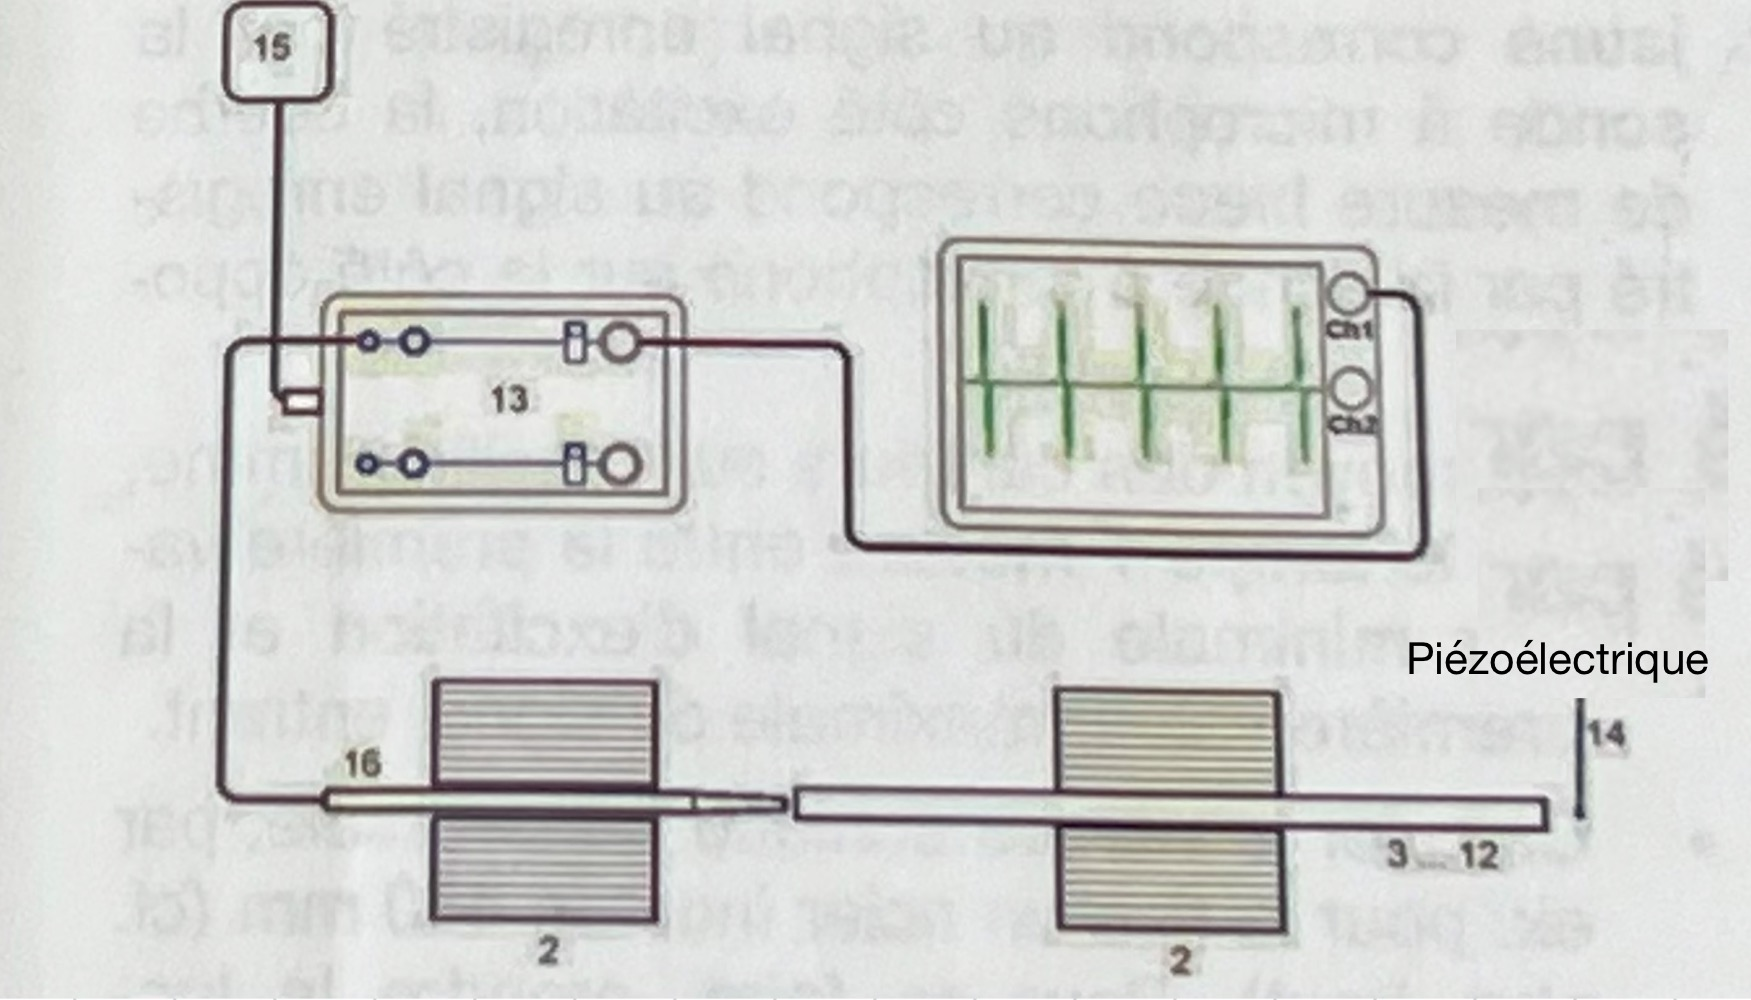
\includegraphics{montage_1.png}}
    \caption{Montage expérimental.~\cite{rapport-heig}}
\end{figure}

\newpage

%Au sein du laboratoire, nous disposons d'un équipement comprenant 
%une boîte renfermant un jeu d'appareillages incluant des tiges 
%d'essai en différents matériaux et de diverses longueurs, 
%deux sondes à microphones, un amplificateur de microphone et 
%d'une alimentation permettant l'enregistrement, 
%l'amplification et l'envoi des signaux de sortie vers un picoscope. 
%De plus, nous disposons de trois tapis de support destinés à maintenir 
%notre propagation d'onde à l'intérieur du solide.

\paragraph{Liste du matériel}
\begin{itemize}
    \item Un générateur piézoélectrique :
    \subitem crée des impulsions qui nous permettent de
    mettre le solide en résonance.\\
    \item Des supports en caoutchouc :
    \subitem permet d'isoler la propagation de l'onde à l'intérieur 
    du solide.\\
    \item Deux sondes à microphone :
    \subitem permettent de mesurer une différence de pression
    créée par le déplacement de l'onde dans le solide.\\
    \item Un amplificateur pour le piézoélectriques :
    \subitem permet d'amplifier la puissance du signal pour le piézoélectrique\\
    \item Une alimentation de secteur :
    \subitem pour le fonctionnement de l'amplificateur.\\
    \item Un PicoScope :
    \subitem transmet l'information mesurée par les microphones
    sur l'ordinateur.\\
    \item Des tiges matériaux de diamètre 10 mm et de longueur différentes :
    \subitem Acier inox 100, 200, 400 mm.
    %\subitem Aluminium 100, 200 mm.
    %\subitem Laiton 100 mm.
    %\subitem Cuivre 100 mm.
    %\subitem Bois dur 200 mm.
    %\subitem PVC 200 mm.
    %\subitem Verre 200 mm.
    %\subitem Verre acrylique 200 mm.
\end{itemize}
\paragraph{Méthode de mesure}
Pour chacune de nos mesures, nous allons régler la bonne fréquence 
d'alimentation grâce à notre générateur de fonction et amplifier la puissance du signal
pour l'injecter dans notre piézoélectrique afin de le faire pulser à la 
fréquence de résonance de notre matériau (voir équation (15)).
À cette fréquence, l'amplitude de notre onde sera la plus grande.
La stimulation continue nous permet de pouvoir prendre une mesure continue
de notre onde sans que la perturbation ne se déforme lors de sa propagation.
Cela nous permet de rester dans le domaine de l'onde progressive.
Le signal capter par notre sonde à microphone et transmis 
à l'aide du PicoScope dans notre ordinateur, nous permet d'afficher notre 
onde. 
En passant par la première équation (voir équation (1)), il nous faut relever la période 
mesurée, qui représente le parcours de l'onde sur un aller-retour de 
notre cylindre. Nous devons ensuite mesurer la longueur de notre 
cylindre à l'aide d'un pied à coulisse. Ces valeurs nous permettent 
de compléter notre équation afin de trouver la célérité dans notre solide.
En passant par la deuxième équation (voir équation (13)), en passant par l'onde plane 
progressive harmonique, nous devons à nouveau utiliser la période 
mesurer précédemment, afin de trouver notre fréquence.
Nous avons besoin de quantifier $k$, pour obtenir notre $\lambda$.

\subsection{\large Résultats / Analyse}
\subsubsection{\large Données brutes}

\paragraph{\large Cylindre Acier inox 400 mm}
\paragraph{Tableau}
\paragraph{Graphe}
\paragraph{Observations}

\newpage

\subsubsection{\large Données réduites}

\paragraph{\large Cylindre Acier inox 400 mm}
\paragraph{Calculs}
\paragraph{Incertitudes}

\newpage

\subsubsection{\large Tableau récapitulatif}
\paragraph{Valeurs}
\paragraph{Incertitudes relatives}
\paragraph{Ecart relatif}

\subsubsection{\large Discussion quantitative}
\paragraph{Incertitude > écart}
validation
\paragraph{Incertitude < écart}
invalidation
discussion critique des méthodes